
\documentclass{article}
\usepackage{graphicx}
\usepackage[top=3cm]{geometry}
\usepackage{tabularray}
\usepackage{afterpage}
\usepackage{amsmath,amssymb}
\usepackage{listings}
\usepackage{subcaption}
\usepackage{mwe}
\usepackage{epstopdf}
\usepackage{textgreek}

\lstset{language=Matlab}
\graphicspath{{./}}
\author{ Harshal Varpe}
\title{ECE 8540 Analysis of Tracking System\\
\Large Lab 6 Report: Particle Filter }

\begin{document}
\maketitle

\section{Introduction}\label{sec:intro}

In this lab report, we deal with the implementation of a particle filter on a given set of data. The filters, such as the Kalman filter or the Extended Kalman filter, can deal with Gaussian noise. Moreover, only the Extended Kalman filter can deal with the non-linear system. But what if the noise is non-gaussian and the system is non-linear? This is where the Particle filter comes into the picture. The particle filter is a Monte Carlo approximation. It needs to be initialized just like the other filters, but many other options, such as proposal distribution, number of particles, when to resample, and resampling method, need to be specified.\\

The measurements are of a system that consists of a 1D position, moving on a line. The motion pattern of the given system is that of an oscillation over a line. The system's sensor detects a field strength that sums up the distances from two fixed-position magnets.

\section{Methods and Implementation}\label{sec:meth}
\subsection{Method}\label{subsec:1}
The particle filter is a continuous cycle of prediction and update. The particle filter works by calculating the next state for each particle. After the calculation, the weights for each particle are derived from the measurement. These weights are then normalized, to sum up to one. After this step, we calculate the desired output or expected value. In the end, we decide if resampling is necessary. If the resampling is performed, then the whole process is repeated.\\

As with all other filters, the first step is to define the model that will be used in this problem. This model includes the following: 
\begin{enumerate}
\item $X_t$, a set of state variables
\item $a_t$, the set of dynamic noises
\item f(), the state transition equation
\item $y_t$, the set of measurements
\item $n_t$, the set of measurement noises
\item g(), the observation equation\\
\end{enumerate}

For this problem, there are two state variables: position and velocity.\\
\begin{equation}
X_t = \begin{bmatrix}
x_t \\
\dot{x}_t
\end{bmatrix}
\label{eq:1}
\end{equation}
Where $x_t$ is the position and $\dot{x_t}$ represents the velocity.\\  

\begin{enumerate}
\item We calculate the next state for each particle $m$ with the following state transition equation.
\begin{equation}
	\lbrace x_t^{(m)} = f(x_{t-1}^{(m)},a_t^{(m)}) \rbrace ^M_{m=1}
	\label{eq:2}
\end{equation}

For our problem, $ f(x_{t-1}^{(m)},a_t^{(m)})$ is given as:
\begin{equation}
f(x_t,a_t) = \begin{bmatrix}
{x_{t+1} = x_t + \dot{x}_t T} \\ \\
\dot{x}_{t+1} = \left\{
\begin{array}{l l}
  2 & \quad \text{if $x_t < -20$} \\
  \dot{x}_t + |a_t| & \quad \text{if $-20 \le x_t < 0$} \\
  \dot{x}_t - |a_t| & \quad \text{if $0 \le x_t \le 20$} \\
  -2 & \quad \text{if $x_t > 20$} \\
\end{array} \right.
\end{bmatrix}
\label{eq:3}
\end{equation}

In the equation \ref{eq:3}, $a_t$ is dynamic noise drawn from a zero-mean Gaussian distribution  $N(0,\sigma_n^2)$. The data was generated using the value of $\sigma_a = 0.0625$.

\item For this problem, Observations are total magnetic strength readings from a sensor.
\begin{equation}
Y_t = \begin{bmatrix} y_t \end{bmatrix}
\label{eq:4}
\end{equation}

\item From the observation equation, we calculate the ideal measurement for the given model.
\begin{equation}
	g(x_t^{(m)},0) = \begin{bmatrix}
	y_t^{(m)} = \frac{1}{\sqrt{2 \pi} \sigma_m}
	\mathrm{exp} ( \frac{-(x_t^{(m)} - x_{m1})^2}{2 \sigma_m^2} ) +
	\frac{1}{\sqrt{2 \pi} \sigma_m}
	\mathrm{exp} ( \frac{-(x_t^{(m)} - x_{m2})^2}{2 \sigma_m^2} )
	\end{bmatrix}
\label{eq:5}
\end{equation}
 For this equation, the value of $x_m1$ and $x_m2$ are -10 and 10, respectively. These variables represent the location of the magnets.

\item We compare the ideal measurement calculated for each particle against the actual measurement. This comparison is made using the following equations:
\begin{equation}
	p(y_t | x_t^{(m)}) = 
	\frac{1}{\sqrt{2 \pi} \sigma_n}
	\mathrm{exp} ( \frac{-(y_t^{(m)} - y_t)^2}{2 \sigma_n^2} )
\label{eq:6}
\end{equation}

\item After comparison between the ideal and actual measurement, we calculate weight updates for each particle using the following equation:

\begin{equation}
\tilde{w}_t^{(m)} = w_{t-1}^{(m)} \cdot p(y_t | x_t^{(m)})
\label{eq:7}
\end{equation}
The calculated weights need to be normalized to sum up to 1. Hence, we do the normalization of weights with the following equation:
\begin{equation}
	w_t^{(m)} = \frac{\tilde{w}_t^{(m)}}{\sum_{m=1}^M \tilde{w}_t^{(m)}}
\label{eq:8}
\end{equation}
 \item Using the updated position state variable and the weight, the expected value or the desired output is calculated.

\begin{equation}
	E[x_t] \approx \sum_{m=1}^M x_t^{(m)} \cdot w_t^{(m)}
\label{eq:9}
\end{equation}

\item After the desired output is calculated, we check if resampling is necessary. To do this, we calculate the coefficient of variation statistic (CV) and effective sampling size(ESS).
\begin{equation}
	CV = \frac{1}{M} \sum_{m=1}^{M}\lbrace M \cdot w^{(m)} - 1 \rbrace ^ 2
\label{eq:10}
\end{equation} 


\begin{equation}
	ESS = \frac{M}{1 + CV}
	\label{eq:11}
\end{equation}
The ESS or effective sample size describes how many particles have appreciable weight. If the number of particles with appreciable weight falls below a certain threshold, then resampling is done. For this problem, the resampling threshold was set at 0.5. This means that if less than 50 percent of the particles have appreciable weight, then we resample.\\

The resampling pseudo-code was provided. This code is given below and is used with minor changes.
\begin{verbatim}
  Assume particle states in P[1...M], weights in W[1...M].

  Q=cumsum(W);          calculate the running totals  
  t=rand(M+1);          t is an array of M+1 uniform random numbers 0 to 1
  T=sort(t);            sort them smallest to largest
  T[M+1]=1.0;           boundary condition for cumulative hist
  i=j=1;                arrays start at 1
  while (i<=M)
    if (T[i] < Q[j])
      Index[i]=j;
      i=i+1;
    else
      j=j+1;
    end if
  end while

  loop (i=1; i<=M; i=i+1)
    NewP[i]=P[index[i]];
    NewW[i]=1/M;
  end loop
\end{verbatim}

\item Loop for time step increment
\end{enumerate}

\subsection{Implementation}\label{subsec:2}
In the previous section, We got the general idea behind the particle filter in multiple steps. In this section, the Matlab implementation of the said steps is explained.
The Matlab code can also be found in the section \ref{sec:apdx}.\\
At the start, the given data is loaded up, and the initial matrices and constants are initialized. The outermost loop runs for the length of a given number of measurements. For this report, this number is 1109. Inside this loop, the estimated state of the system is calculated for each particle. The estimated state is a vector used to plot the plots in section \ref{sec:res}. After the state estimation, the CV and ESS calculations are done. Depending on the resampling threshold and ESS value, a decision is made on whether to resample.\\
To understand when resampling is done, and the effect of resampling on particles, the plots of position vs weights are plotted before and after resampling.\\

\section{Result}\label{sec:res}

The figure\ref{fig:1} shows the raw measurement data given. The sensor recorded the total magnetic strength as it passed by the two magnets. As we can see from the figure, the sensor readings are quite noisy.\\
\begin{figure}[!ht]
\centering
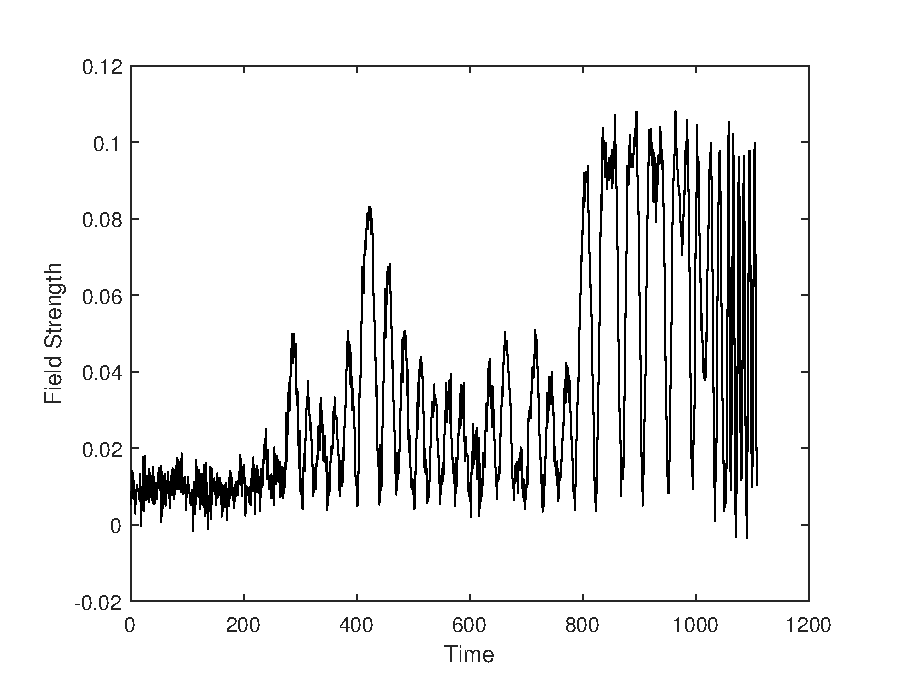
\includegraphics[scale=0.6]{measurement_data.eps}
\caption{Plot of Raw Sensor data}
\label{fig:1}
\end{figure}

Let us now take a look at the workings of the particle filter. We know that in the particle filter, particles are resampled after the number of irrelevant points increases.
Consider plots 1a and 1b. Both plots show particle position against their weights for a single instance. Before resampling (plot 1a), we can see that most particles are between positions -2.5 and -1. This means that the probability that the actual position is between -2.5 to -1 is high. However, we are still not sure where exactly between -2.5 and -1. Hence, we resample and get new particles with zero weights. This is what we observe in plot 1b. We initiate new points between the positions -2.5 and -1.\\

Let us consider plots 2a and 2b. In plot 2a, we see most particles between positions 2.5 to 4. Also, the particles at position 3 seem to have the highest weights. Therefore, we initialize new points between 2.5 to 4, with more points near position 3. The weights after resampling will be zero until we recalculate the weight for these new particles in the next iteration. Moreover, in these plots, we notice two bell curves indicating the non-gaussian nature. We can make similar observations about plots 3a and 3b.\\


\begin{figure}
\centering
\begin{subfigure}{.6\textwidth}
    \centering
    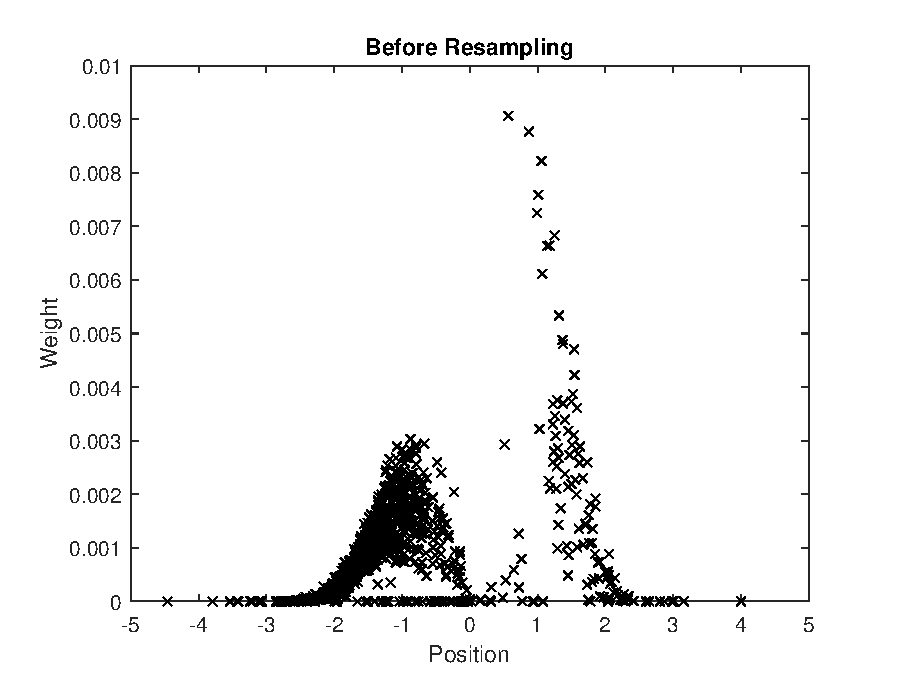
\includegraphics[scale=0.6]{before_sampling_1.eps}
	\subcaption{1a}
\end{subfigure}%
\begin{subfigure}{.6\textwidth}
    \centering
    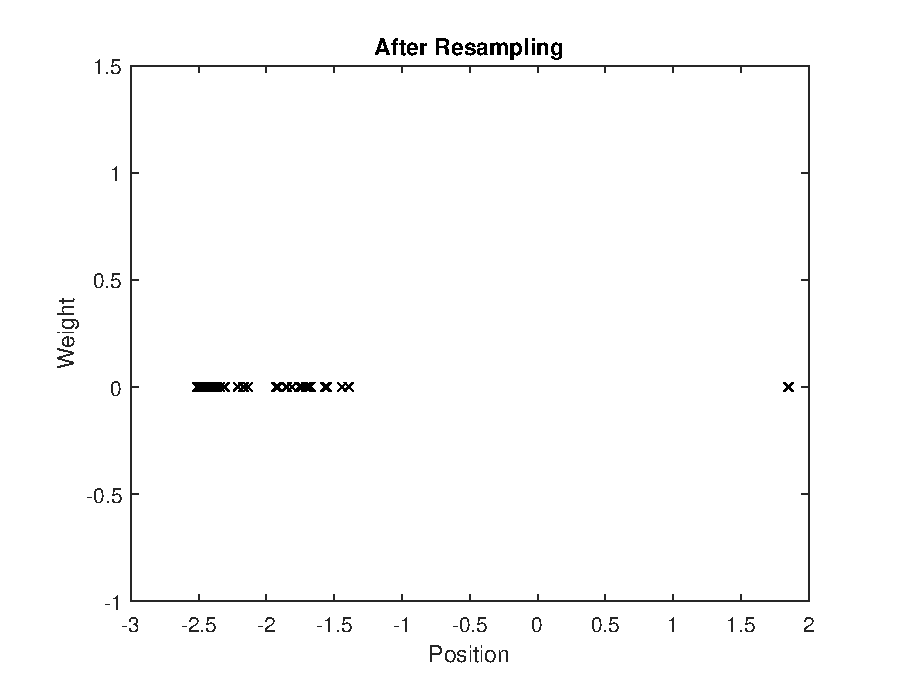
\includegraphics[scale=0.6]{after_sampling_1.eps}
\subcaption{1b}
\end{subfigure}
\begin{subfigure}{.6\textwidth}
    \centering
    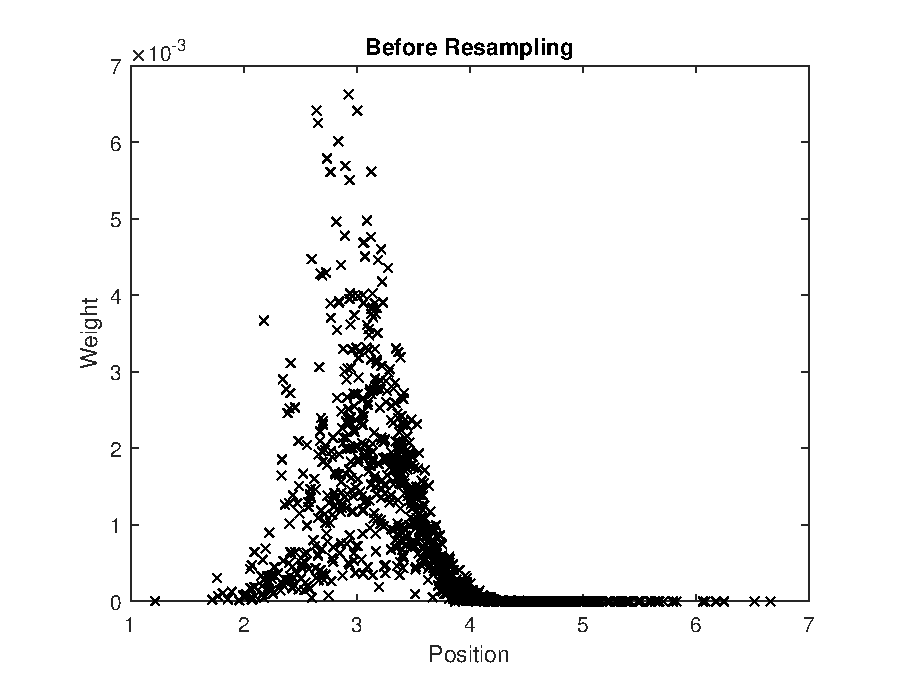
\includegraphics[scale=0.6]{before_sampling_2.eps}
\subcaption{2a}
\end{subfigure}%
\begin{subfigure}{.6\textwidth}
    \centering
    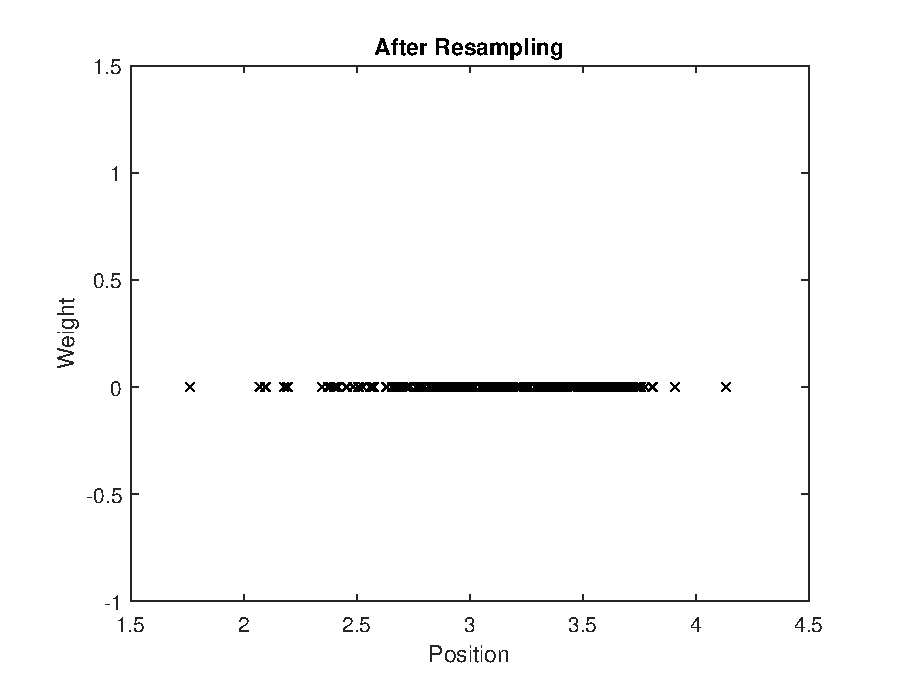
\includegraphics[scale=0.6]{after_sampling_2.eps}
\subcaption{2b}
\end{subfigure}
\begin{subfigure}{0.6\textwidth}
    \centering
    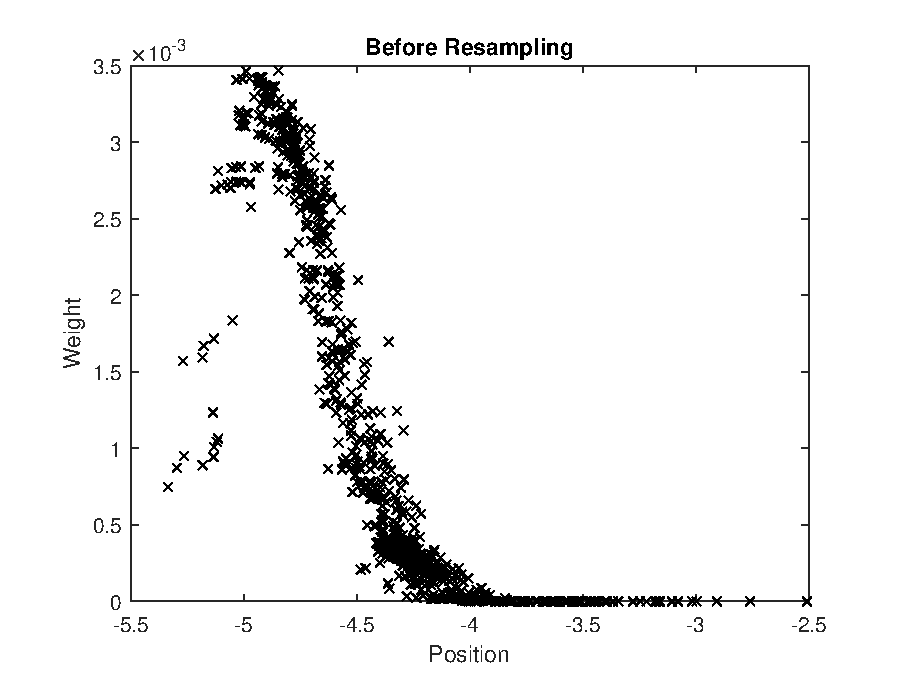
\includegraphics[scale=0.6]{before_sampling_3.eps}
\subcaption{3a}
\end{subfigure}%
\begin{subfigure}{0.6\textwidth}
    \centering
    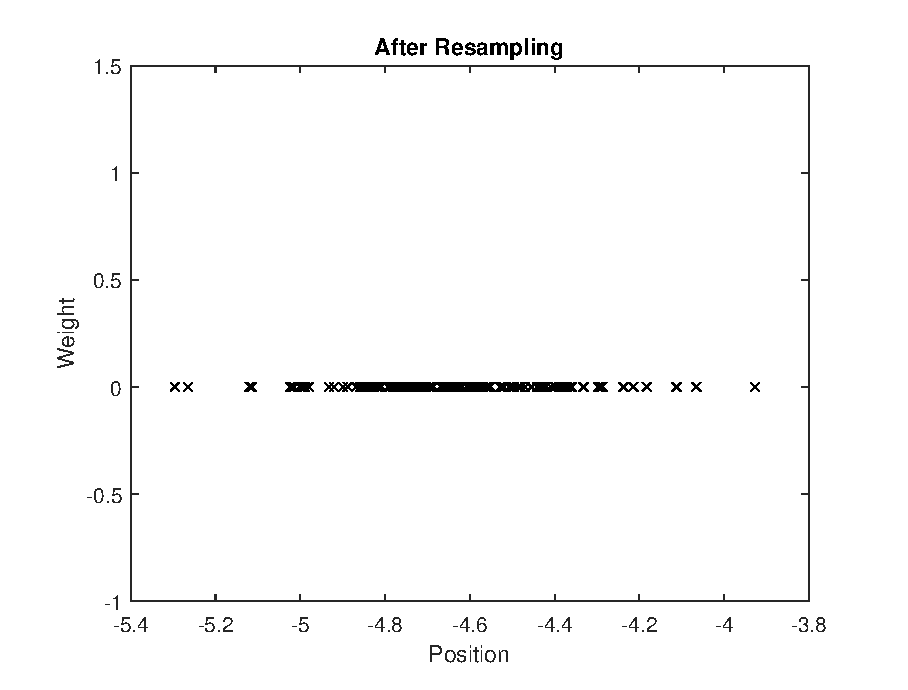
\includegraphics[scale=0.6]{after_sampling_3.eps}
\subcaption{3b}
\end{subfigure}
\caption[short]{Plot of particle position against their corresponding weights before and after resampling.}
\end{figure}

In figure \ref{fig:2}, we can see the plot of the true position against the estimated position calculated using the Particle filter. We can see that the filter takes a few iterations to perform properly. However, after the initial errors, the estimates follow the ground truth very closely as evident from the graph.

\begin{figure}
\centering
\includegraphics[scale=0.6]{result.eps}
\caption{Plot of True position against estimated position}
\label{fig:2}
\end{figure}

\pagebreak
\clearpage
\section{Conclusion}\label{sec:conc}

In this lab, we learned how the particle filter estimates the state of a complex system with noisy measurements. The particle filter is better equipped to handle the non-linear system with non-gaussian noise.\\

We read about how resampling is one of the best features of the particle filter. However, we can see from the plots in section \ref{sec:res}, how the resampling exactly takes place and why it takes place. As the particle filter iterations take place, the number of particles with bad weights is reduced. In contrast, the number of particles with good/appreciable weights around the probable positions increases.


\section{Apendix}\label{sec:apdx}
\begin{lstlisting}[frame=single]
clear
clc
close all
% --------------------------------------------------------------------------
data = importdata("magnets_data.txt");

gt_pos = data(:,1);
gt_vel = data(:,2);
gt_sensor = data(:,3);

% Partical Filter Variables
M = 1000; %number of particles
sig_a = 0.0625; % Variance of dynamic noise
sig_m = 4;
sig_n = 0.003906; % variance of measurement noise
Xm1 = -10; % position of magnet
Xm2 = 10;   % position of magnet

% Initialization of weights and state variables
x_pos = zeros(M,1);
x_vel = zeros(M,1);
x_pos_prev = zeros(M,1);
x_vel_prev = zeros(M,1);

wt_norm = 1/M * zeros(M,1);
wt_prev = 1/M * ones(M,1);
wt_up = 1/M * zeros(M,1);

index = zeros(M,1);
x_pos_1 = zeros(M,1);
x_vel_1 = zeros(M,1);
wt_norm_1 = zeros(M,1);

%plot flags
resampling_count = 0
wt_plt = 0; %weight plots
resample_plt = 50; % resampling plots will start at this point

%resampling threshold
rs_thresh = 0.5 ;

X1 = 1:length(gt_sensor);
X2 = 1:M;

result = zeros(length(gt_sensor),1);


q = 2000;
for i = 1:length(gt_sensor)
%     E(i) = 0;

    for j = 1:1:M
        x_pos(j) = x_pos_prev(j) + x_vel_prev(j);
        if(x_pos_prev(j) < -20)
            x_vel(i) = 2;
            
        elseif(x_pos_prev(j) >= -20 && x_pos_prev(j) < 0 )
            x_vel(j) = x_vel_prev(j) + abs(normrnd(0,sig_a));
            
        elseif(x_pos_prev(j) >= 0 && x_pos_prev(j) <= 20)
            x_vel(j) = x_vel_prev(j) - abs(normrnd(0,sig_a));
            
        elseif(x_pos_prev(j) > 20)
            x_vel(j) = -2;
        end
        
        y_t = ( (1/(sqrt(2*pi)*sig_m)) * exp((-(x_pos_prev(j)-Xm1)^2) / (2*sig_m^2)) ) + (1/(sqrt(2*pi)*sig_m)) * exp(-(x_pos_prev(j)-Xm2)^2 / (2 *(sig_m^2)) );
        
        %weight updates via ideal measurement
        p = (1/(sqrt(2*pi)*sig_n)) * exp (-(y_t-gt_sensor(i))^2 / (2 * sig_n^2)) ;
        
        wt_up(j) = wt_prev(j) *  p;        
        wt_prev(j) = wt_up(j);
        x_pos_prev(j) = x_pos(j);
        x_vel_prev(j) = x_vel(j);
    end
    %weight normalization
    wt_norm = wt_up ./ sum(wt_up);
%     sum(wt_up)
    E =0 ;
    for k = 1:M
        E = E + (wt_norm(k) * x_pos(k));
%         E(i) = E(i) + wt_norm(k) + x_pos(k);
    end
    
    result(i) = E;
    
    CV = 0;

    for k = 1:M
        CV = CV + (M*wt_norm(k) - 1)^2;
    end
    
    CV = CV/M;
    ESS = M/(1+CV);
    
    
    if ESS < rs_thresh*M
        
        if(wt_plt > 0)
            figure(i)
            plot(x_pos, wt_norm,'kx')
            xlabel('Position');
            ylabel('Weight');
            title("Before Resampling")
        end
        
        resampling_count = resampling_count + 1
        if resampling_count >= resample_plt || resampling_count <= resample_plt + 2
            wt_plt = 1;
        end
        
        Q = cumsum(wt_norm);
        t = rand(M+1,1);
        T = sort(t);
        T(M+1) = 1;
        x=1;
        y=1;
        while x<=M
           
            if T(x) < Q(y)
               index(x) = y;
               x = x+1;
           else
               y=y+1;
           end
        end
        for x = 1:M
            x_pos(x)      = x_pos(index(x));
            x_pos_prev(x)  = x_pos_prev(index(x));

            x_vel(x)        = x_vel(index(x));
            x_vel_prev(x)    = x_vel_prev(index(x)) ;

            wt_norm(x)          = 1/M;
            wt_prev(x)     = 1/M;
        end
%            for x=1:M
%                x_pos_1(x) = x_pos(index(x));
%                wt_norm_1(x) = 1/M;
%                x_vel_1(x) = x_vel(index(x));
%            end
%         x_pos = x_pos_1;
%         wt_norm = wt_norm_1;
%         x_vel = x_vel_1;
        if(wt_plt > 0)
            figure(i+100)
            plot(x_pos, wt_norm,'kx')
            xlabel('Position');
            ylabel('Weight');
            title("After Resampling")
%             q = q+1;
        end
    end
%     wt_prev = wt_norm; % uncmnt this blokc it works
%     x_pos_prev = x_pos;
%     x_vel_prev = x_vel;

    if resampling_count > resample_plt
        wt_plt = 0;
    end


end
figure(i+1)
plot(gt_pos,"kx")
hold on
plot(result,"k-")
xlabel("Time")
ylabel("Position")
legend("Ground truth","Estimated Position")

hold off
figure(i+2)
plot(gt_sensor)
xlabel("Time")
ylabel("Field Strength")
\end{lstlisting}


\end{document}